\documentclass[]{article}
\usepackage{lmodern}
\usepackage{amssymb,amsmath}
\usepackage{ifxetex,ifluatex}
\usepackage{fixltx2e} % provides \textsubscript
\ifnum 0\ifxetex 1\fi\ifluatex 1\fi=0 % if pdftex
  \usepackage[T1]{fontenc}
  \usepackage[utf8]{inputenc}
\else % if luatex or xelatex
  \ifxetex
    \usepackage{mathspec}
  \else
    \usepackage{fontspec}
  \fi
  \defaultfontfeatures{Ligatures=TeX,Scale=MatchLowercase}
\fi
% use upquote if available, for straight quotes in verbatim environments
\IfFileExists{upquote.sty}{\usepackage{upquote}}{}
% use microtype if available
\IfFileExists{microtype.sty}{%
\usepackage{microtype}
\UseMicrotypeSet[protrusion]{basicmath} % disable protrusion for tt fonts
}{}
\usepackage[margin=1in]{geometry}
\usepackage{hyperref}
\hypersetup{unicode=true,
            pdftitle={R Markdown},
            pdfauthor={UNSW},
            pdfborder={0 0 0},
            breaklinks=true}
\urlstyle{same}  % don't use monospace font for urls
\usepackage{color}
\usepackage{fancyvrb}
\newcommand{\VerbBar}{|}
\newcommand{\VERB}{\Verb[commandchars=\\\{\}]}
\DefineVerbatimEnvironment{Highlighting}{Verbatim}{commandchars=\\\{\}}
% Add ',fontsize=\small' for more characters per line
\usepackage{framed}
\definecolor{shadecolor}{RGB}{248,248,248}
\newenvironment{Shaded}{\begin{snugshade}}{\end{snugshade}}
\newcommand{\AlertTok}[1]{\textcolor[rgb]{0.94,0.16,0.16}{#1}}
\newcommand{\AnnotationTok}[1]{\textcolor[rgb]{0.56,0.35,0.01}{\textbf{\textit{#1}}}}
\newcommand{\AttributeTok}[1]{\textcolor[rgb]{0.77,0.63,0.00}{#1}}
\newcommand{\BaseNTok}[1]{\textcolor[rgb]{0.00,0.00,0.81}{#1}}
\newcommand{\BuiltInTok}[1]{#1}
\newcommand{\CharTok}[1]{\textcolor[rgb]{0.31,0.60,0.02}{#1}}
\newcommand{\CommentTok}[1]{\textcolor[rgb]{0.56,0.35,0.01}{\textit{#1}}}
\newcommand{\CommentVarTok}[1]{\textcolor[rgb]{0.56,0.35,0.01}{\textbf{\textit{#1}}}}
\newcommand{\ConstantTok}[1]{\textcolor[rgb]{0.00,0.00,0.00}{#1}}
\newcommand{\ControlFlowTok}[1]{\textcolor[rgb]{0.13,0.29,0.53}{\textbf{#1}}}
\newcommand{\DataTypeTok}[1]{\textcolor[rgb]{0.13,0.29,0.53}{#1}}
\newcommand{\DecValTok}[1]{\textcolor[rgb]{0.00,0.00,0.81}{#1}}
\newcommand{\DocumentationTok}[1]{\textcolor[rgb]{0.56,0.35,0.01}{\textbf{\textit{#1}}}}
\newcommand{\ErrorTok}[1]{\textcolor[rgb]{0.64,0.00,0.00}{\textbf{#1}}}
\newcommand{\ExtensionTok}[1]{#1}
\newcommand{\FloatTok}[1]{\textcolor[rgb]{0.00,0.00,0.81}{#1}}
\newcommand{\FunctionTok}[1]{\textcolor[rgb]{0.00,0.00,0.00}{#1}}
\newcommand{\ImportTok}[1]{#1}
\newcommand{\InformationTok}[1]{\textcolor[rgb]{0.56,0.35,0.01}{\textbf{\textit{#1}}}}
\newcommand{\KeywordTok}[1]{\textcolor[rgb]{0.13,0.29,0.53}{\textbf{#1}}}
\newcommand{\NormalTok}[1]{#1}
\newcommand{\OperatorTok}[1]{\textcolor[rgb]{0.81,0.36,0.00}{\textbf{#1}}}
\newcommand{\OtherTok}[1]{\textcolor[rgb]{0.56,0.35,0.01}{#1}}
\newcommand{\PreprocessorTok}[1]{\textcolor[rgb]{0.56,0.35,0.01}{\textit{#1}}}
\newcommand{\RegionMarkerTok}[1]{#1}
\newcommand{\SpecialCharTok}[1]{\textcolor[rgb]{0.00,0.00,0.00}{#1}}
\newcommand{\SpecialStringTok}[1]{\textcolor[rgb]{0.31,0.60,0.02}{#1}}
\newcommand{\StringTok}[1]{\textcolor[rgb]{0.31,0.60,0.02}{#1}}
\newcommand{\VariableTok}[1]{\textcolor[rgb]{0.00,0.00,0.00}{#1}}
\newcommand{\VerbatimStringTok}[1]{\textcolor[rgb]{0.31,0.60,0.02}{#1}}
\newcommand{\WarningTok}[1]{\textcolor[rgb]{0.56,0.35,0.01}{\textbf{\textit{#1}}}}
\usepackage{longtable,booktabs}
\usepackage{graphicx,grffile}
\makeatletter
\def\maxwidth{\ifdim\Gin@nat@width>\linewidth\linewidth\else\Gin@nat@width\fi}
\def\maxheight{\ifdim\Gin@nat@height>\textheight\textheight\else\Gin@nat@height\fi}
\makeatother
% Scale images if necessary, so that they will not overflow the page
% margins by default, and it is still possible to overwrite the defaults
% using explicit options in \includegraphics[width, height, ...]{}
\setkeys{Gin}{width=\maxwidth,height=\maxheight,keepaspectratio}
\IfFileExists{parskip.sty}{%
\usepackage{parskip}
}{% else
\setlength{\parindent}{0pt}
\setlength{\parskip}{6pt plus 2pt minus 1pt}
}
\setlength{\emergencystretch}{3em}  % prevent overfull lines
\providecommand{\tightlist}{%
  \setlength{\itemsep}{0pt}\setlength{\parskip}{0pt}}
\setcounter{secnumdepth}{0}
% Redefines (sub)paragraphs to behave more like sections
\ifx\paragraph\undefined\else
\let\oldparagraph\paragraph
\renewcommand{\paragraph}[1]{\oldparagraph{#1}\mbox{}}
\fi
\ifx\subparagraph\undefined\else
\let\oldsubparagraph\subparagraph
\renewcommand{\subparagraph}[1]{\oldsubparagraph{#1}\mbox{}}
\fi

%%% Use protect on footnotes to avoid problems with footnotes in titles
\let\rmarkdownfootnote\footnote%
\def\footnote{\protect\rmarkdownfootnote}

%%% Change title format to be more compact
\usepackage{titling}

% Create subtitle command for use in maketitle
\providecommand{\subtitle}[1]{
  \posttitle{
    \begin{center}\large#1\end{center}
    }
}

\setlength{\droptitle}{-2em}

  \title{R Markdown}
    \pretitle{\vspace{\droptitle}\centering\huge}
  \posttitle{\par}
    \author{UNSW}
    \preauthor{\centering\large\emph}
  \postauthor{\par}
      \predate{\centering\large\emph}
  \postdate{\par}
    \date{2019}


\begin{document}
\maketitle

\hypertarget{the-bigger-picture}{%
\section{The Bigger Picture}\label{the-bigger-picture}}

In this document we learn how to create and manipulate R Markdown
documents. Simply put, we are learning how to create documents,
slideshows, websites and reports to showcase our work with data science.
In the overall context of the workflow, this falls into the category of
producing our presentations.

~

\hypertarget{what-is-r-markdown}{%
\section{What is R Markdown?}\label{what-is-r-markdown}}

\begin{quote}
\href{https://www.lynda.com/RStudio-tutorials/What-Markdown/699348/2700131-4.html?srchtrk=index\%3a1\%0alinktypeid\%3a2\%0aq\%3ar+markdown\%0apage\%3a1\%0as\%3arelevance\%0asa\%3atrue\%0aproducttypeid\%3a2}{Lynda
1.1}
\end{quote}

\begin{quote}
\href{https://www.lynda.com/RStudio-tutorials/What-R-Markdown/699348/2800209-4.html?srchtrk=index\%3a1\%0alinktypeid\%3a2\%0aq\%3ar+markdown\%0apage\%3a1\%0as\%3arelevance\%0asa\%3atrue\%0aproducttypeid\%3a2}{Lynda
1.2}
\end{quote}

\hypertarget{markup-languages}{%
\subsection{Markup Languages}\label{markup-languages}}

\begin{itemize}
\tightlist
\item
  R Markdown is a markup language
\item
  Markup langauges are systems for annotating documents and other media
\item
  Some other markup languages are:

  \begin{itemize}
  \tightlist
  \item
    Markdown (different from R Markdown!)
  \item
    LaTeX
  \item
    HTML
  \end{itemize}
\end{itemize}

\hypertarget{how-does-r-markdown-work}{%
\subsection{How does R Markdown work?}\label{how-does-r-markdown-work}}

\begin{itemize}
\tightlist
\item
  R Markdown begins by looking like a weird R script with its own
  special syntax
\item
  R Markdown documents have the special file extension \texttt{.Rmd}
\item
  It includes chunks of R code, and possibly some snippets of other
  languages
\item
  After we ``knit'' the document together (according to how we specify),
  it looks like a nicely rendered form of media
\item
  The document you are currently reading was built in R Markdown!
\end{itemize}

\hypertarget{what-can-r-markdown-do}{%
\subsection{What can R Markdown do?}\label{what-can-r-markdown-do}}

There are three broad types of documents R Markdown can produce. Note
that each have sub-categories, and other document types exist. See
\href{https://rmarkdown.rstudio.com/lesson-9.html}{here} for more
information.

\hypertarget{pdf}{%
\subsubsection{PDF}\label{pdf}}

\begin{quote}
\href{https://www.lynda.com/RStudio-tutorials/Writing-PDF-reports-R-Markdown/699348/2800210-4.html?srchtrk=index\%3a1\%0alinktypeid\%3a2\%0aq\%3ar+markdown\%0apage\%3a1\%0as\%3arelevance\%0asa\%3atrue\%0aproducttypeid\%3a2}{Lynda
1.3}
\end{quote}

\begin{itemize}
\tightlist
\item
  These documents always look the same
\item
  They cannot be edited without leaving a `footprint' (the edits will be
  noticeable!)
\item
  They can be password protected
\end{itemize}

\hypertarget{html-reports}{%
\subsubsection{HTML Reports}\label{html-reports}}

\begin{quote}
\href{https://www.lynda.com/RStudio-tutorials/Writing-HTML-reports-R-Markdown/699348/2801126-4.html?srchtrk=index\%3a1\%0alinktypeid\%3a2\%0aq\%3ar+markdown\%0apage\%3a1\%0as\%3arelevance\%0asa\%3atrue\%0aproducttypeid\%3a2}{Lynda
1.4}
\end{quote}

\begin{itemize}
\tightlist
\item
  Documents which can be put online
\item
  They are easily viewable on mobile
\item
  These reports can interact with htmlwidgets (moving objects,
  responsive to the viewers clicks!)
\end{itemize}

\hypertarget{html-presentations}{%
\subsubsection{HTML Presentations}\label{html-presentations}}

\begin{quote}
\href{https://www.lynda.com/RStudio-tutorials/Writing-HTML-presentations-R-Markdown/699348/2801127-4.html?srchtrk=index\%3a1\%0alinktypeid\%3a2\%0aq\%3ar+markdown\%0apage\%3a1\%0as\%3arelevance\%0asa\%3atrue\%0aproducttypeid\%3a2}{Lynda
1.5}
\end{quote}

\begin{itemize}
\tightlist
\item
  These are HTML documents comparable to a slideshow presentation
\item
  There are several preset styles
\item
  Some styles are very customisable
\end{itemize}

\hypertarget{other-media}{%
\subsubsection{Other Media}\label{other-media}}

\begin{quote}
\href{https://www.lynda.com/RStudio-tutorials/What-else-can-you-build-R-Markdown/699348/2800211-4.html?srchtrk=index\%3a1\%0alinktypeid\%3a2\%0aq\%3ar+markdown\%0apage\%3a1\%0as\%3arelevance\%0asa\%3atrue\%0aproducttypeid\%3a2}{Lynda
1.6}
\end{quote}

R Markdown can also produce:

\begin{itemize}
\tightlist
\item
  Microsoft PowerPoint presentations
\item
  Microsoft Word documents
\item
  Blog-style webpages (Blogdown)
\item
  Multi-chapter books and reference documents (Bookdown)
\end{itemize}

\hypertarget{latex-bibtex-and-tex}{%
\section{LaTeX, BibTeX and TeX}\label{latex-bibtex-and-tex}}

\begin{quote}
\href{https://www.lynda.com/RStudio-tutorials/What-LaTeX-BibTeX/699348/2700132-4.html?srchtrk=index\%3a1\%0alinktypeid\%3a2\%0aq\%3ar+markdown\%0apage\%3a1\%0as\%3arelevance\%0asa\%3atrue\%0aproducttypeid\%3a2}{Lynda
2.1}
\end{quote}

\hypertarget{latex}{%
\subsection{LaTeX}\label{latex}}

\begin{itemize}
\tightlist
\item
  LaTeX is a markup language like R Markdown
\item
  It is heavily used in academia for its ability to create mathematical
  formulae with ease and precision
\item
  We can call LaTeX in R Markdown if we configure RStudio correctly
\end{itemize}

\hypertarget{bibtex}{%
\subsection{BibTeX}\label{bibtex}}

\begin{itemize}
\tightlist
\item
  A reference management software for LaTeX
\item
  It is required to customise the appearance and layout of all PDF
  documents in R Markdown
\end{itemize}

\hypertarget{tex}{%
\subsection{TeX}\label{tex}}

\begin{itemize}
\tightlist
\item
  A typesetting system which encompasses LaTeX
\item
  Developed with LaTeX partly to process mathematical formulae
\item
  LaTeX is \textbf{one distribution} of TeX
\end{itemize}

\hypertarget{installing-tex}{%
\section{Installing TeX}\label{installing-tex}}

\begin{quote}
\href{https://www.lynda.com/RStudio-tutorials/Setting-up-TeX-generating-R-Markdown-reports/699348/2801128-4.html?srchtrk=index\%3a1\%0alinktypeid\%3a2\%0aq\%3ar+markdown\%0apage\%3a1\%0as\%3arelevance\%0asa\%3atrue\%0aproducttypeid\%3a2}{Lynda
2.2}
\end{quote}

This installation is needed to call upon several functions of R
Markdown. Depending on your operating system, the installation for TeX
will be one of these options:

\begin{longtable}[]{@{}ccc@{}}
\toprule
\begin{minipage}[b]{0.30\columnwidth}\centering
macOS\strut
\end{minipage} & \begin{minipage}[b]{0.30\columnwidth}\centering
Linux\strut
\end{minipage} & \begin{minipage}[b]{0.30\columnwidth}\centering
Windows\strut
\end{minipage}\tabularnewline
\midrule
\endhead
\begin{minipage}[t]{0.30\columnwidth}\centering
Go to \url{http://www.tug.org/mactex} and install TeX\strut
\end{minipage} & \begin{minipage}[t]{0.30\columnwidth}\centering
Run \texttt{sudo\ apt-get\ install\ texlive-full}\strut
\end{minipage} & \begin{minipage}[t]{0.30\columnwidth}\centering
Go to \url{https://miktex.org/download} and install TeX\strut
\end{minipage}\tabularnewline
\bottomrule
\end{longtable}

After the installation, RStudio will automatically be able to detect TeX
on your computer.

\hypertarget{installing-pandoc}{%
\section{Installing Pandoc}\label{installing-pandoc}}

\begin{quote}
\href{https://www.lynda.com/RStudio-tutorials/Installing-Pandoc/699348/2700133-4.html?srchtrk=index\%3a1\%0alinktypeid\%3a2\%0aq\%3ar+markdown\%0apage\%3a1\%0as\%3arelevance\%0asa\%3atrue\%0aproducttypeid\%3a2}{Lynda
2.3}
\end{quote}

\begin{itemize}
\tightlist
\item
  Pandoc is a software which can convert files from one markup format to
  another
\item
  This is what will convert our \texttt{.Rmd} (R Markdown) files to
  other, more useful formats
\item
  Make sure the latest version of Pandoc is installed on your computer
  by visiting \url{https://pandoc.org/installing.html}
\end{itemize}

\hypertarget{the-r-markdown-package}{%
\section{The R Markdown Package}\label{the-r-markdown-package}}

\begin{quote}
\href{https://www.lynda.com/RStudio-tutorials/Installing-R-Markdown/699348/2801129-4.html?srchtrk=index\%3a1\%0alinktypeid\%3a2\%0aq\%3ar+markdown\%0apage\%3a1\%0as\%3arelevance\%0asa\%3atrue\%0aproducttypeid\%3a2}{Lynda
3.1}
\end{quote}

R Markdown is necessary to install as a package through R Studio by
running the following:

\begin{Shaded}
\begin{Highlighting}[]
\KeywordTok{install.packages}\NormalTok{(}\StringTok{"rmarkdown"}\NormalTok{)}
\end{Highlighting}
\end{Shaded}

\begin{itemize}
\tightlist
\item
  R Markdown is now almost up and running
\item
  The final step is to watch for RStudio warning that extra packages
  need to be installed for R Markdown to operate
\item
  A pop-up may or may not appear, depending on the current version of
  \texttt{rmarkdown}
\end{itemize}

Once these are installed, R Markdown is ready for use!

\hypertarget{the-r-markdown-interface}{%
\section{The R Markdown interface}\label{the-r-markdown-interface}}

\begin{quote}
\href{https://www.lynda.com/RStudio-tutorials/R-Markdown-knitting-generating-outputs/699348/2801130-4.html?srchtrk=index\%3a1\%0alinktypeid\%3a2\%0aq\%3ar+markdown\%0apage\%3a1\%0as\%3arelevance\%0asa\%3atrue\%0aproducttypeid\%3a2}{Lynda
3.2}
\end{quote}

\textbf{Reminder: R Markdown files are of the type \texttt{.Rmd}}

\begin{itemize}
\tightlist
\item
  When we're in RStudio, we create a new R Markdown document
\item
  It is recommended to do this in a new (or existing) \emph{R Project}
\item
  Navigate to
  \texttt{File}\(\rightarrow\)\texttt{New\ File}\(\rightarrow\)\texttt{Rmarkdown...}
\item
  This menu will appear.
\end{itemize}

\begin{itemize}
\tightlist
\item
  We are immediately forced to make a choice, however, no selection we
  make is permanent
\item
  By default, we will begin by working in an HTML document
\item
  When we select OK, we have an R Markdown document in front of us
\end{itemize}

\begin{itemize}
\tightlist
\item
  If we save this document, it will appear in our files tab
\end{itemize}

\begin{itemize}
\tightlist
\item
  The document currently appears to look like a script
\item
  We use the ``Knit'' button to compile this script into the document
  type we chose
\end{itemize}

~

\begin{itemize}
\tightlist
\item
  We are also able to freely modify the text in the \texttt{.Rmd} file
\item
  This is our first step to creating our own reports
\end{itemize}

\hypertarget{the-yaml-header}{%
\section{The YAML Header}\label{the-yaml-header}}

\begin{quote}
\href{https://www.lynda.com/RStudio-tutorials/YAML-header-Rmd-file/699348/2801131-4.html?srchtrk=index\%3a1\%0alinktypeid\%3a2\%0aq\%3ar+markdown\%0apage\%3a1\%0as\%3arelevance\%0asa\%3atrue\%0aproducttypeid\%3a2}{Lynda
3.3}
\end{quote}

\begin{itemize}
\tightlist
\item
  YAML is a standard for configuration files
\item
  By modifying the ``YAML header'', we configure how our R Markdown file
  is configured
\item
  The YAML header is everything between the two \texttt{-\/-\/-}
\item
  It is automatically generated when we create a document
\item
  In this format, indentation matters, so when we modify our headers we
  must be careful
\end{itemize}

\hypertarget{basic-options}{%
\subsection{Basic options:}\label{basic-options}}

\begin{itemize}
\tightlist
\item
  The \texttt{title}, \texttt{author} and \texttt{date} options are
  self-explanatory
\item
  The \texttt{output} option dictates the document we produce when we
  Knit (by default it is set to whatever we selected when creating the
  document)
\item
  Some output styles (which we will cover) are:

  \begin{itemize}
  \tightlist
  \item
    html\_document
  \item
    pdf\_document
  \item
    slidy\_presentation
  \item
    ioslides\_presentation
  \item
    beamer\_presentation
  \end{itemize}
\end{itemize}

\hypertarget{additional-options}{%
\subsection{Additional options:}\label{additional-options}}

\begin{itemize}
\tightlist
\item
  There are very many different fields we can add to the YAML header
\item
  Some are simple to include and require only one line, such as the
  \texttt{subtitle} field added below
\item
  Others are more complex and must be formatted by several layers of
  indentation, such as the \texttt{toc} field
\end{itemize}

\begin{itemize}
\tightlist
\item
  We will introduce a few more fields later on, but here are lists of
  \href{https://bookdown.org/yihui/rmarkdown/pdf-document.html}{useful
  PDF-relevant fields} and
  \href{https://bookdown.org/yihui/rmarkdown/html-document.html}{useful
  HTML-relevant fields}
\end{itemize}

\hypertarget{code-chunks}{%
\section{Code Chunks}\label{code-chunks}}

\begin{quote}
\href{https://www.lynda.com/RStudio-tutorials/Code-chunks-global-code-chunk-settings/699348/2800212-4.html?srchtrk=index\%3a1\%0alinktypeid\%3a2\%0aq\%3ar+markdown\%0apage\%3a1\%0as\%3arelevance\%0asa\%3atrue\%0aproducttypeid\%3a2}{Lynda
3.4}
\end{quote}

R Markdown is enormously useful for its ability to display and run code.

\hypertarget{creating-code-chunks}{%
\subsection{Creating Code Chunks}\label{creating-code-chunks}}

\begin{Shaded}
\begin{Highlighting}[]
\NormalTok{text <-}\StringTok{ "R Markdown is cool"}
\KeywordTok{print}\NormalTok{(text)}
\end{Highlighting}
\end{Shaded}

\begin{verbatim}
## [1] "R Markdown is cool"
\end{verbatim}

\begin{Shaded}
\begin{Highlighting}[]
\NormalTok{x =}\StringTok{ }\KeywordTok{seq}\NormalTok{(}\OperatorTok{-}\DecValTok{5}\NormalTok{,}\DecValTok{5}\NormalTok{,}\FloatTok{0.1}\NormalTok{)}
\NormalTok{y =}\StringTok{ }\NormalTok{x}\OperatorTok{^}\DecValTok{2}
\KeywordTok{plot}\NormalTok{(x,y)}
\end{Highlighting}
\end{Shaded}

\begin{figure}

{\centering 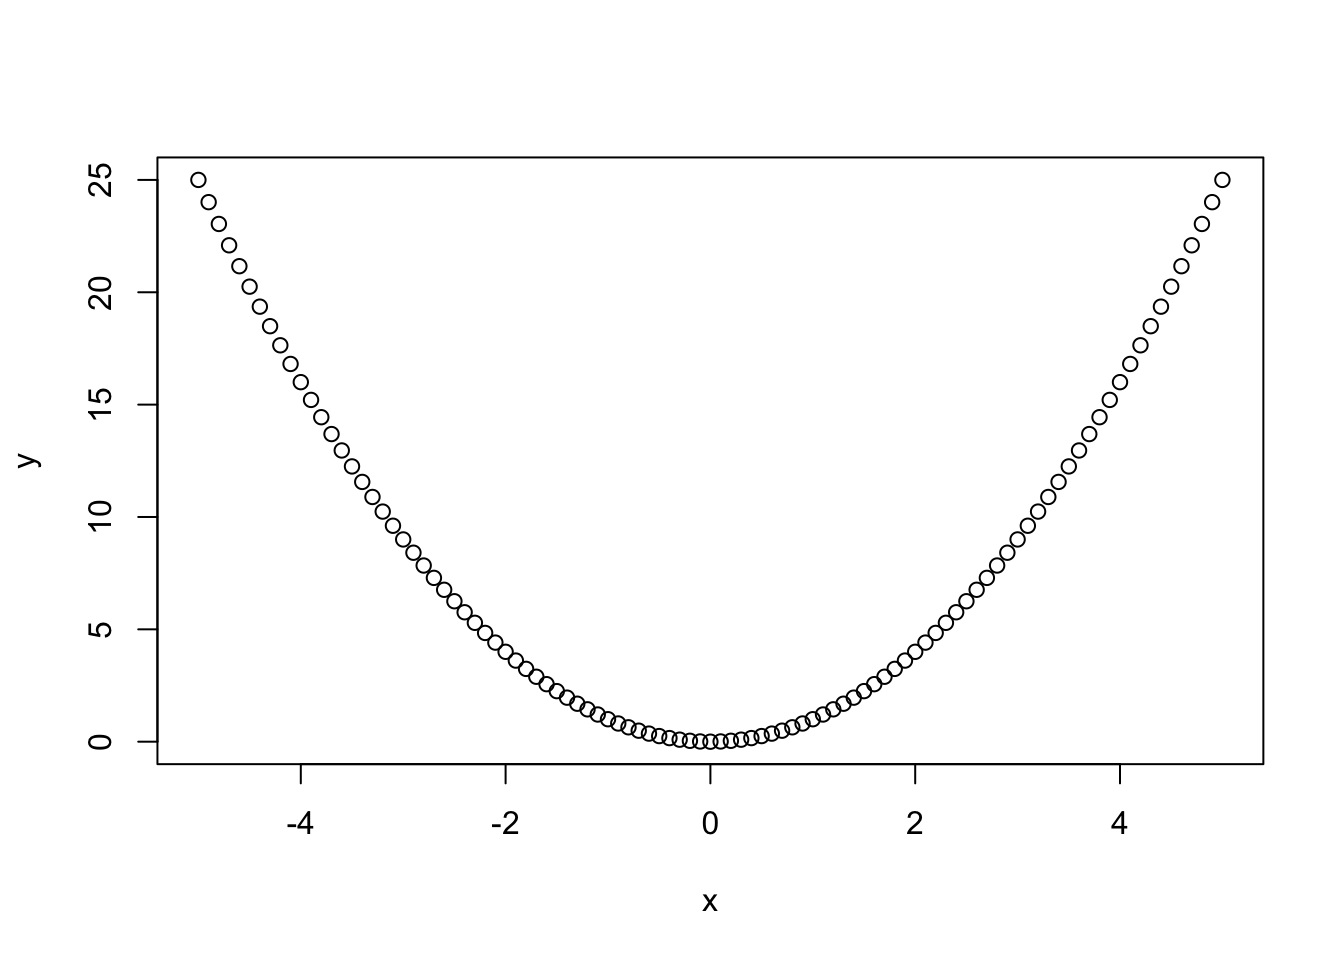
\includegraphics[width=0.4\linewidth]{RMarkdown_files/figure-latex/code1-1} 

}

\caption{*Fig 1: A nice parabola.*}\label{fig:code1}
\end{figure}

\begin{itemize}
\tightlist
\item
  ``Code chunks'' are small, dedicated sections of the R Markdown
  document which come with their own options for displaying or running
  code
\item
  We begin a code chunk with three backticks (`s) and end it with three
  backticks
\item
  After the three backticks we have a section of curly brackets
  (\texttt{\{\ \}})
\item
  In these backticks, we state the language we are coding in, then type
  a space, then name the code chunk
\item
  \textbf{Warning}: never give two code chunks in the same document the
  same name, or the document will not compile
\end{itemize}

\begin{itemize}
\tightlist
\item
  The above code runs and produces the code shown above
\end{itemize}

\hypertarget{code-chunk-options}{%
\subsection{Code Chunk options}\label{code-chunk-options}}

\hypertarget{global-chunk-options}{%
\subsubsection{Global Chunk options}\label{global-chunk-options}}

\begin{itemize}
\tightlist
\item
  When creating chunks, all options are set to a ``global'' default
  which spans the entire document
\item
  These default options are specified in the chunk called
  \texttt{setup}, which is automatically generated at the beginning of
  our \texttt{.Rmd} file
\item
  The \texttt{opts\_chunk\$set()} function can set any default chunk
  options, and we can modify this to include whatever options we need
\end{itemize}

\hypertarget{local-chunk-options}{%
\subsubsection{Local Chunk options}\label{local-chunk-options}}

\begin{itemize}
\tightlist
\item
  Local chunk options are specified from within one chunk and are listed
  in the curly brackets (\texttt{\{\ \}})
\item
  They overwrite global options
\end{itemize}

\hypertarget{list-of-options}{%
\subsubsection{List of options}\label{list-of-options}}

\begin{longtable}[]{@{}cc@{}}
\toprule
Option & Argument\tabularnewline
\midrule
\endhead
\texttt{include} & TRUE or FALSE\tabularnewline
\texttt{echo} & TRUE or FALSE\tabularnewline
\texttt{message} & TRUE or FALSE\tabularnewline
\texttt{warning} & TRUE or FALSE\tabularnewline
\texttt{out.width} & ``40\%'' or 300px\tabularnewline
\texttt{fig.cap} & ``Caption''\tabularnewline
\texttt{fig.align} & `center', etc\tabularnewline
\bottomrule
\end{longtable}

\href{https://yihui.name/knitr/options/\#plots}{For the long, full list
of options, see this link.}

\hypertarget{running-code-in-r-markdown-documents}{%
\section{Running code in R Markdown
documents}\label{running-code-in-r-markdown-documents}}

\begin{quote}
\href{https://www.lynda.com/RStudio-tutorials/Writing-running-R-code-R-Markdown-files/699348/2700134-4.html?srchtrk=index\%3a1\%0alinktypeid\%3a2\%0aq\%3ar+markdown\%0apage\%3a1\%0as\%3arelevance\%0asa\%3atrue\%0aproducttypeid\%3a2}{Lynda
3.5}
\end{quote}

\hypertarget{specifying-output}{%
\subsection{Specifying output}\label{specifying-output}}

We can choose how code output is displayed in RStudio.

\begin{itemize}
\tightlist
\item
  We go to the ``cog'' icon and we can select from displaying output
  inline or in console
\end{itemize}

Output inline VS output in console:

\hypertarget{running-individual-lines}{%
\subsection{Running individual lines}\label{running-individual-lines}}

\begin{itemize}
\tightlist
\item
  To run individual lines is the same as in an R script
\item
  If a line has been selected, CTRL+ENTER will run the line
\end{itemize}

\hypertarget{running-from-chunks}{%
\subsection{Running from chunks}\label{running-from-chunks}}

\begin{itemize}
\tightlist
\item
  There are two buttons in every code chunk
\item
  The first runs all code above a chunk

  \begin{itemize}
  \tightlist
  \item
    This is very useful if lots of our code is inter-dependent
  \end{itemize}
\item
  The second runs just the current chunk
\end{itemize}

\hypertarget{the-run-button}{%
\subsection{The Run button}\label{the-run-button}}

\begin{itemize}
\tightlist
\item
  This button prodivdes a list of options for running chunks
\end{itemize}

\hypertarget{sectioning-r-markdown-documents}{%
\section{Sectioning R Markdown
documents}\label{sectioning-r-markdown-documents}}

\begin{quote}
\href{https://www.lynda.com/RStudio-tutorials/Splitting-documents-sections-slides-R-Markdown/699348/2700135-4.html?srchtrk=index\%3a1\%0alinktypeid\%3a2\%0aq\%3ar+markdown\%0apage\%3a1\%0as\%3arelevance\%0asa\%3atrue\%0aproducttypeid\%3a2}{Lynda
3.6}
\end{quote}

\hypertarget{sectioning-in-standard-documents}{%
\subsection{Sectioning in standard
documents}\label{sectioning-in-standard-documents}}

\begin{itemize}
\tightlist
\item
  In R Markdown, the hash (\texttt{\#}) symbol is used for headings
\item
  One hash, \#, is an `h1' heading (the largest)
\item
  Two hashes, \#\#, is an `h2' heading (slightly less large)
\item
  This goes all the way to six hashes, \#\#\#\#\#\#, for the smallest
  subheading
\item
  Each heading can be formatted to be different (see \texttt{.css} files
  below), but by default, the more ``sub'' the heading is, the smaller
  the font
\end{itemize}

Our R Markdown code VS its PDF output VS its HTML output

\hypertarget{sectioning-in-slides}{%
\subsection{Sectioning in slides}\label{sectioning-in-slides}}

\begin{itemize}
\tightlist
\item
  If we are working with a slideshow document, headings and the hash
  (\texttt{\#}) symbol also serve as slide headings
\item
  As an example, we can do this in the \texttt{slidy\_presentation}
  format (discussed below)
\end{itemize}

\hypertarget{tabsets}{%
\section{Tabsets}\label{tabsets}}

\begin{quote}
\href{https://www.lynda.com/RStudio-tutorials/Tabbed-sections-R-Markdown-HTML-reports/699348/2700136-4.html?srchtrk=index\%3a1\%0alinktypeid\%3a2\%0aq\%3ar+markdown\%0apage\%3a1\%0as\%3arelevance\%0asa\%3atrue\%0aproducttypeid\%3a2}{Lynda
3.7}
\end{quote}

\begin{itemize}
\tightlist
\item
  \textbf{Note}: this will \textbf{\emph{only}} work with the
  \texttt{html\_document} formatting
\item
  Tabset options can create sophisticated headings
\item
  If we write \texttt{\{.tabset\}} immediately after a heading, the
  subheadings will be condensed into a selection bar
\end{itemize}

\begin{itemize}
\tightlist
\item
  If we write \texttt{\{.tabset\ .tabset-dropdown\}}, this selection bar
  will be a dropdown menu instead
\end{itemize}

\hypertarget{r-markdown-text-options}{%
\section{R Markdown text options}\label{r-markdown-text-options}}

\begin{quote}
\href{https://www.lynda.com/RStudio-tutorials/Formatting-text-R-Markdown-files/699348/2700137-4.html?srchtrk=index\%3a1\%0alinktypeid\%3a2\%0aq\%3ar+markdown\%0apage\%3a1\%0as\%3arelevance\%0asa\%3atrue\%0aproducttypeid\%3a2}{Lynda
3.8} and
\href{https://www.lynda.com/RStudio-tutorials/Bullets-lists-R-Markdown/699348/2801132-4.html?srchtrk=index\%3a1\%0alinktypeid\%3a2\%0aq\%3ar+markdown\%0apage\%3a1\%0as\%3arelevance\%0asa\%3atrue\%0aproducttypeid\%3a2}{Lynda
3.9}
\end{quote}

\begin{longtable}[]{@{}ll@{}}
\toprule
\begin{minipage}[b]{0.47\columnwidth}\raggedright
Feature\strut
\end{minipage} & \begin{minipage}[b]{0.47\columnwidth}\raggedright
Implementation\strut
\end{minipage}\tabularnewline
\midrule
\endhead
\begin{minipage}[t]{0.47\columnwidth}\raggedright
Bold\strut
\end{minipage} & \begin{minipage}[t]{0.47\columnwidth}\raggedright
Surround text by \texttt{**} or \texttt{\_\_}\strut
\end{minipage}\tabularnewline
\begin{minipage}[t]{0.47\columnwidth}\raggedright
Italics\strut
\end{minipage} & \begin{minipage}[t]{0.47\columnwidth}\raggedright
Surround text by \texttt{*}\strut
\end{minipage}\tabularnewline
\begin{minipage}[t]{0.47\columnwidth}\raggedright
Strikethrough\strut
\end{minipage} & \begin{minipage}[t]{0.47\columnwidth}\raggedright
Surround text by \texttt{\textasciitilde{}\textasciitilde{}}\strut
\end{minipage}\tabularnewline
\begin{minipage}[t]{0.47\columnwidth}\raggedright
Superscript\strut
\end{minipage} & \begin{minipage}[t]{0.47\columnwidth}\raggedright
Surround text by \texttt{\^{}}\strut
\end{minipage}\tabularnewline
\begin{minipage}[t]{0.47\columnwidth}\raggedright
Code font\strut
\end{minipage} & \begin{minipage}[t]{0.47\columnwidth}\raggedright
Surround text by backticks (`s)\strut
\end{minipage}\tabularnewline
\begin{minipage}[t]{0.47\columnwidth}\raggedright
Bullet points\strut
\end{minipage} & \begin{minipage}[t]{0.47\columnwidth}\raggedright
\texttt{-} then space at the beginning of a line, and repeat on the next
line\strut
\end{minipage}\tabularnewline
\begin{minipage}[t]{0.47\columnwidth}\raggedright
Sub-bullet points\strut
\end{minipage} & \begin{minipage}[t]{0.47\columnwidth}\raggedright
Four spaces, then \texttt{-} at the beginning of a line, and repeat on
the next line\strut
\end{minipage}\tabularnewline
\begin{minipage}[t]{0.47\columnwidth}\raggedright
Numbered list\strut
\end{minipage} & \begin{minipage}[t]{0.47\columnwidth}\raggedright
\texttt{1.} then space at the beginning of the line, and repeat on the
next line (type the number one (1) repeatedly!)\strut
\end{minipage}\tabularnewline
\begin{minipage}[t]{0.47\columnwidth}\raggedright
New paragraph\strut
\end{minipage} & \begin{minipage}[t]{0.47\columnwidth}\raggedright
Two spaces at the end of a line\strut
\end{minipage}\tabularnewline
\bottomrule
\end{longtable}

Here's an
\href{https://www.rstudio.com/wp-content/uploads/2015/02/rmarkdown-cheatsheet.pdf}{R
Markdown cheat sheet} to help remember all these formats!

\hypertarget{code-chunk-navigation-and-naming-convention}{%
\section{Code Chunk Navigation and Naming
Convention}\label{code-chunk-navigation-and-naming-convention}}

\begin{quote}
\href{https://www.lynda.com/RStudio-tutorials/Name-your-code-chunks-sensibly/699348/2801133-4.html?srchtrk=index\%3a1\%0alinktypeid\%3a2\%0aq\%3ar+markdown\%0apage\%3a1\%0as\%3arelevance\%0asa\%3atrue\%0aproducttypeid\%3a2}{Lynda
4.1}
\end{quote}

\begin{itemize}
\tightlist
\item
  Technically, R Markdown does not require any code chunks to be named
\item
  It is, however, always a good idea to name code chunks for debugging
  and readability purposes
\item
  The \texttt{namer} package can be installed to automatically name
  chunks in a script
\item
  However, for large scripts, naming code chunks appropriately is the
  recommended approach
\item
  This makes navigation through an \texttt{.Rmd} file much easier
\end{itemize}

As an example, consider a very large \texttt{.Rmd} file containing
material on the \texttt{ggplot} package:

The button at the bottom of the script tab provides instand navigation
between headings and code chunks in an \texttt{.Rmd} file. This
navigation becomes much clearer with appropriate code chunk names.

\hypertarget{including-code-from-script-files}{%
\section{Including Code from Script
Files}\label{including-code-from-script-files}}

\begin{quote}
\href{https://www.lynda.com/RStudio-tutorials/Including-code-from-script-files/699348/2700138-4.html?srchtrk=index\%3a1\%0alinktypeid\%3a2\%0aq\%3ar+markdown\%0apage\%3a1\%0as\%3arelevance\%0asa\%3atrue\%0aproducttypeid\%3a2}{Lynda
4.2}
\end{quote}

\begin{itemize}
\tightlist
\item
  If we have a script file saved in our project folder, we can call on
  it with the \texttt{source()} command
\end{itemize}

\begin{Shaded}
\begin{Highlighting}[]
\KeywordTok{source}\NormalTok{(}\StringTok{"script.R"}\NormalTok{)}
\end{Highlighting}
\end{Shaded}

\begin{verbatim}
## [1] "I have been called from script.R!"
\end{verbatim}

\hypertarget{different-slide-formats}{%
\section{Different Slide Formats}\label{different-slide-formats}}

\begin{quote}
\href{https://www.lynda.com/RStudio-tutorials/Including-code-from-script-files/699348/2700138-4.html?srchtrk=index\%3a1\%0alinktypeid\%3a2\%0aq\%3ar+markdown\%0apage\%3a1\%0as\%3arelevance\%0asa\%3atrue\%0aproducttypeid\%3a2}{Lynda
5.1}
\end{quote}

There are three types of slides formats R Markdown, with their own
strengths and weaknesses:

\begin{itemize}
\tightlist
\item
  Ioslides (\texttt{output:\ ioslides\_presentation})
\item
  Slidy (\texttt{output:\ slidy\_presentation})
\item
  Beamer (\texttt{output:\ beamer\_presentation})
\end{itemize}

Ioslides and Slidy produce HTML output whereas Beamer produces PDF
output.

\hypertarget{ioslides}{%
\subsection{Ioslides}\label{ioslides}}

\begin{quote}
\href{https://www.lynda.com/RStudio-tutorials/Features-ioslides-presentations/699348/2700140-4.html?srchtrk=index\%3a1\%0alinktypeid\%3a2\%0aq\%3ar+markdown\%0apage\%3a1\%0as\%3arelevance\%0asa\%3atrue\%0aproducttypeid\%3a2}{Lynda
5.2}
\end{quote}

\begin{itemize}
\tightlist
\item
  Creates HTML slides
\item
  Designed by Google for their 2010 I/O conference
\item
  Almost no customisability
\item
  Works well on mobile
\item
  Built in with hotkey functions:
\end{itemize}

\begin{longtable}[]{@{}cc@{}}
\toprule
Hotkey & Effect\tabularnewline
\midrule
\endhead
\texttt{w} & Toggle to widescreen\tabularnewline
\texttt{o} & Toggle to overview\tabularnewline
\texttt{h} & Highlight code line\tabularnewline
\texttt{p} & Include presenter notes\tabularnewline
\bottomrule
\end{longtable}

Highlighting lines of code requires the use of this unique syntax:

Creating presenter notes (slides that can only be shown by pressing
\texttt{p}) requires wrapping the content by some HTML:

\hypertarget{slidy}{%
\subsection{Slidy}\label{slidy}}

\begin{quote}
\href{https://www.lynda.com/RStudio-tutorials/Features-Slidy-presentations/699348/2700141-4.html?srchtrk=index\%3a1\%0alinktypeid\%3a2\%0aq\%3ar+markdown\%0apage\%3a1\%0as\%3arelevance\%0asa\%3atrue\%0aproducttypeid\%3a2}{Lynda
5.3}
\end{quote}

\begin{itemize}
\tightlist
\item
  Creates HTML slides
\item
  Slidy is the best choice for making custom HTML slides with custom
  \texttt{.css} files
\item
  By default they are very minimal
\item
  Also built with hotkeys
\end{itemize}

\begin{longtable}[]{@{}cc@{}}
\toprule
Hotkey & Effect\tabularnewline
\midrule
\endhead
\texttt{c} & Opens a table of contents\tabularnewline
\texttt{a} & Converts the slides to a linear document\tabularnewline
\texttt{s} & Makes font smaller\tabularnewline
\texttt{b} & Makes font bigger\tabularnewline
\texttt{f} & Removes the footer\tabularnewline
\bottomrule
\end{longtable}

By manipulating the YAML header, we can add a timer to the footer:

\begin{verbatim}
output:
  slidy_presentation:
    duration: 2
\end{verbatim}

Here is a set of Slidy slides produced with and without custom
\texttt{.css} styles:

\href{https://github.com/alblaine/countess/blob/master/styles.css}{Credit
to alblaine} for the style!

\hypertarget{beamer}{%
\subsection{Beamer}\label{beamer}}

\begin{quote}
\href{https://www.lynda.com/RStudio-tutorials/PDF-presentations-Beamer/699348/2801134-4.html?srchtrk=index\%3a1\%0alinktypeid\%3a2\%0aq\%3ar+markdown\%0apage\%3a1\%0as\%3arelevance\%0asa\%3atrue\%0aproducttypeid\%3a2}{Lynda
5.4}
\end{quote}

\begin{itemize}
\tightlist
\item
  Creates PDF slides
\item
  Based on the LaTeX class ``Beamer''
\item
  Many different styles are available online
\item
  Knowledge of LaTeX is required to do certain features, such as
  including slide numbers
\end{itemize}

Here is the default Beamer VS one with custom styles:

Including custom styles is achieved in two steps:

\begin{enumerate}
\def\labelenumi{\arabic{enumi}.}
\tightlist
\item
  Modifying the YAML header as such
\end{enumerate}

\begin{verbatim}
output:
  beamer_presentation:
    includes:
      in_header: styles/styles.tex
\end{verbatim}

\begin{enumerate}
\def\labelenumi{\arabic{enumi}.}
\setcounter{enumi}{1}
\tightlist
\item
  Creating a \texttt{.tex} file in our project in the directory
  \texttt{slides/styles.tex}
\end{enumerate}

These few commands (written in your LaTeX file) will allow you to make a
few changes to your slides:

\begin{itemize}
\tightlist
\item
  Add custom colours and themes to your slides
\item
  Go to \href{http://deic.uab.es/~iblanes/beamer_gallery/}{the Beamer
  gallery} to find themes and colours you like!
\end{itemize}

\begin{verbatim}
\usetheme{THEME_NAME}
\usecolortheme{COLOUR_THEME_NAME}
\end{verbatim}

\begin{itemize}
\tightlist
\item
  Add slide numbers to your slides
\end{itemize}

\begin{verbatim}
\setbeamertemplate{navigation symbols}{}
\setbeamertemplate{footline}[page number]
\end{verbatim}

\hypertarget{controlling-chart-output}{%
\section{Controlling Chart Output}\label{controlling-chart-output}}

\begin{quote}
\href{https://www.lynda.com/RStudio-tutorials/ggplot2-plots-R-Markdown-documents/699348/2800213-4.html?srchtrk=index\%3a1\%0alinktypeid\%3a2\%0aq\%3ar+markdown\%0apage\%3a1\%0as\%3arelevance\%0asa\%3atrue\%0aproducttypeid\%3a2}{Lynda
6.1 - 6.3}
\end{quote}

\begin{itemize}
\tightlist
\item
  We produce graphs in R Markdown by putting the relevant code in code
  chunks and then running them
\item
  This works with normal code and \texttt{ggplot2} code
\end{itemize}

\begin{Shaded}
\begin{Highlighting}[]
\CommentTok{# Base R plot}
\NormalTok{x =}\StringTok{ }\KeywordTok{seq}\NormalTok{(}\OperatorTok{-}\DecValTok{5}\NormalTok{,}\DecValTok{5}\NormalTok{,}\FloatTok{0.1}\NormalTok{)}
\NormalTok{y =}\StringTok{ }\NormalTok{x}\OperatorTok{^}\DecValTok{2}
\KeywordTok{plot}\NormalTok{(x,y)}

\CommentTok{# ggplot2 plot}
\KeywordTok{library}\NormalTok{(}\StringTok{"tidyverse"}\NormalTok{)}
\end{Highlighting}
\end{Shaded}

\begin{center}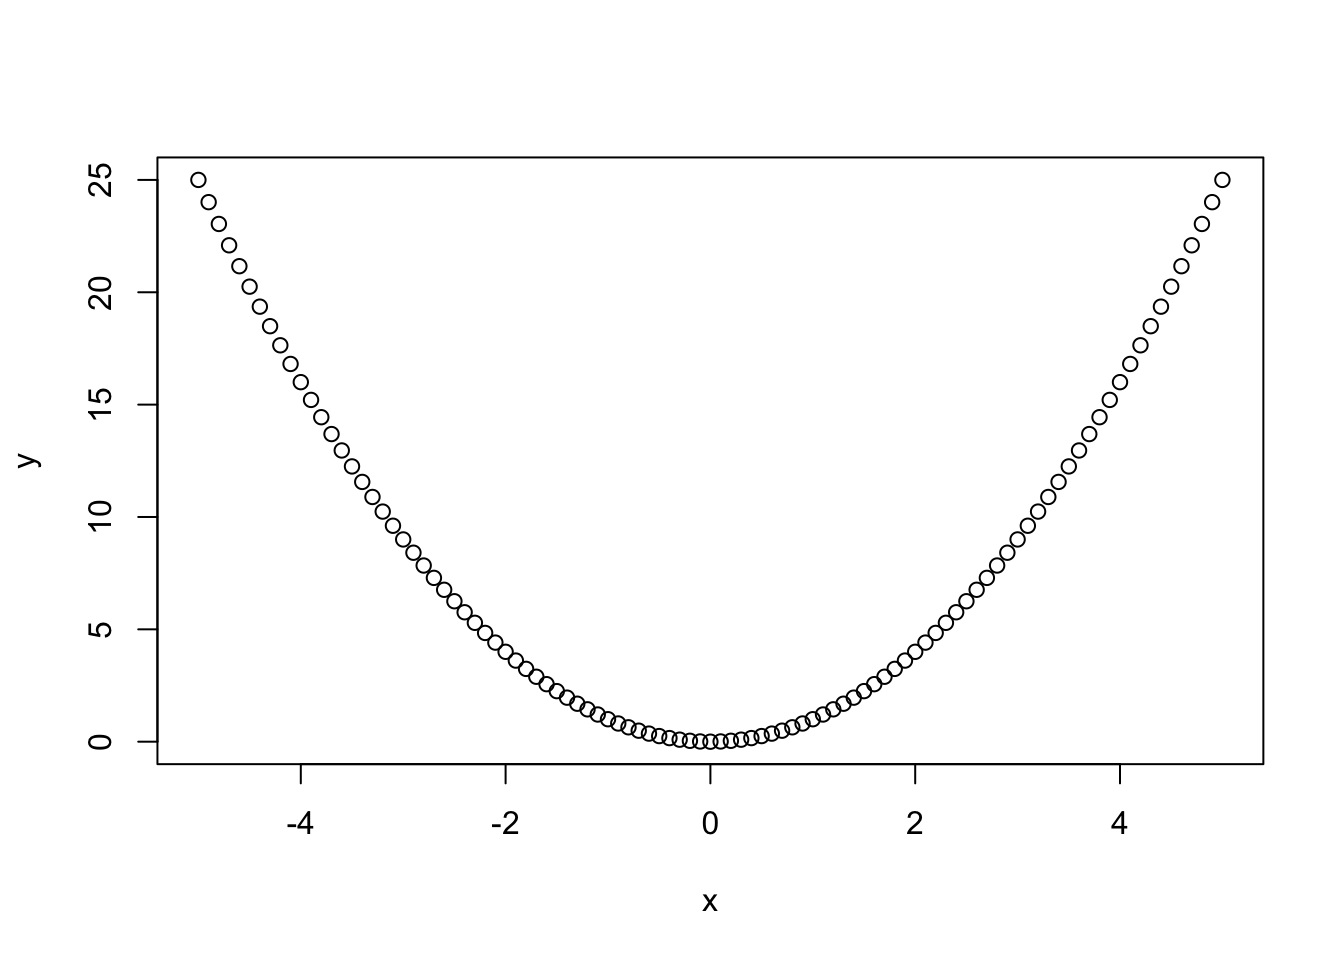
\includegraphics[width=0.6\linewidth]{RMarkdown_files/figure-latex/chart_output1-1} \end{center}

\begin{Shaded}
\begin{Highlighting}[]
\KeywordTok{load}\NormalTok{(}\StringTok{"tidy_EnvAcc_data/consumption.rdata"}\NormalTok{)}
\NormalTok{consumption }\OperatorTok
\StringTok{  }\KeywordTok{ggplot}\NormalTok{() }\OperatorTok{+}
\StringTok{  }\KeywordTok{geom_col}\NormalTok{(}\KeywordTok{aes}\NormalTok{(}\DataTypeTok{x =}\NormalTok{ year,}
               \DataTypeTok{y =}\NormalTok{ water_consumption,}
               \DataTypeTok{fill =}\NormalTok{ State))}
\end{Highlighting}
\end{Shaded}

\begin{center}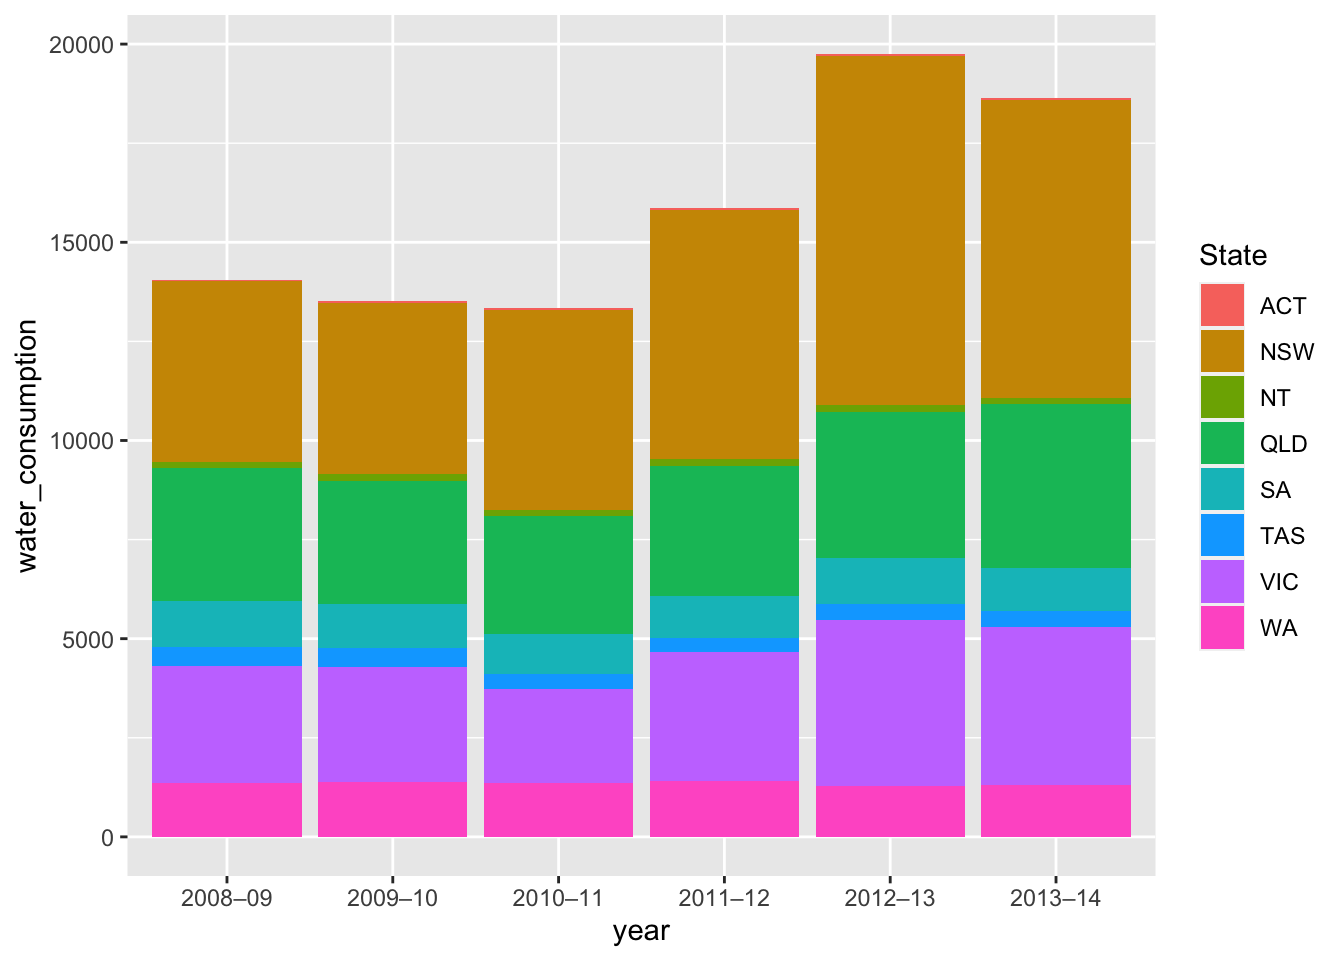
\includegraphics[width=0.6\linewidth]{RMarkdown_files/figure-latex/chart_output1-2} \end{center}

\texttt{fig.width} and \texttt{fig.height} can only take numeric
arguments, and one or both can be specified. Measurements are in inches.
Generally used for PDF.

\begin{center}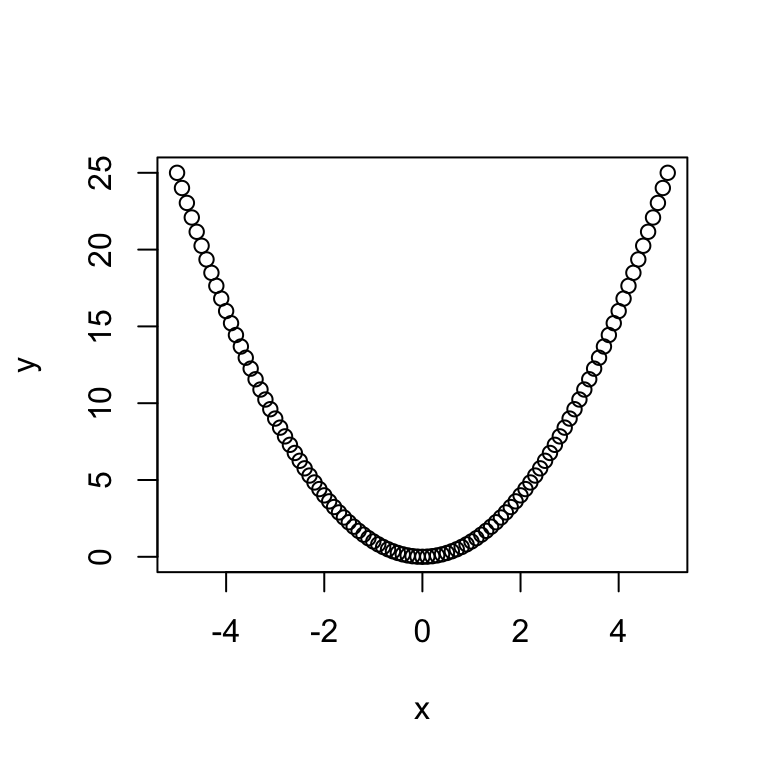
\includegraphics[width=0.6\linewidth]{RMarkdown_files/figure-latex/chart_output2-1} \end{center}

\texttt{fig.width} and \texttt{fig.asp} (also numeric, often between 0
and 1) can both be specified, and figure height will be determined based
on \texttt{fig.asp}.

\begin{center}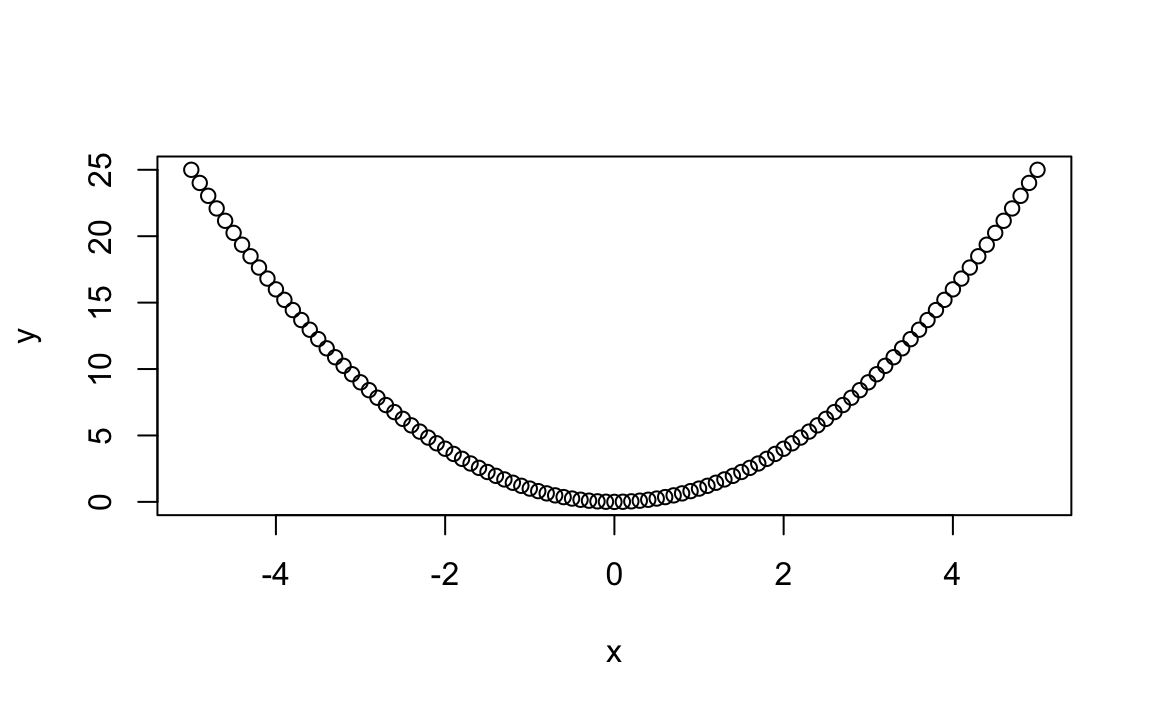
\includegraphics[width=0.6\linewidth]{RMarkdown_files/figure-latex/chart_output3-1} \end{center}

\texttt{out.width} and \texttt{out.height} can take several arguments.
Generally we use a character string to specify percentage or pixel
measurement (eg out.width = ``40\%'' or out.width = ``480px''). However,
\texttt{out.height} cannot overwrite the aspect ratio, and so it has
limited usefulness.

Take note that these options can take some special LaTeX arguments as
well. See \href{https://yihui.name/knitr/options/\#plots}{here under
``out.width, out.height''}.

\begin{center}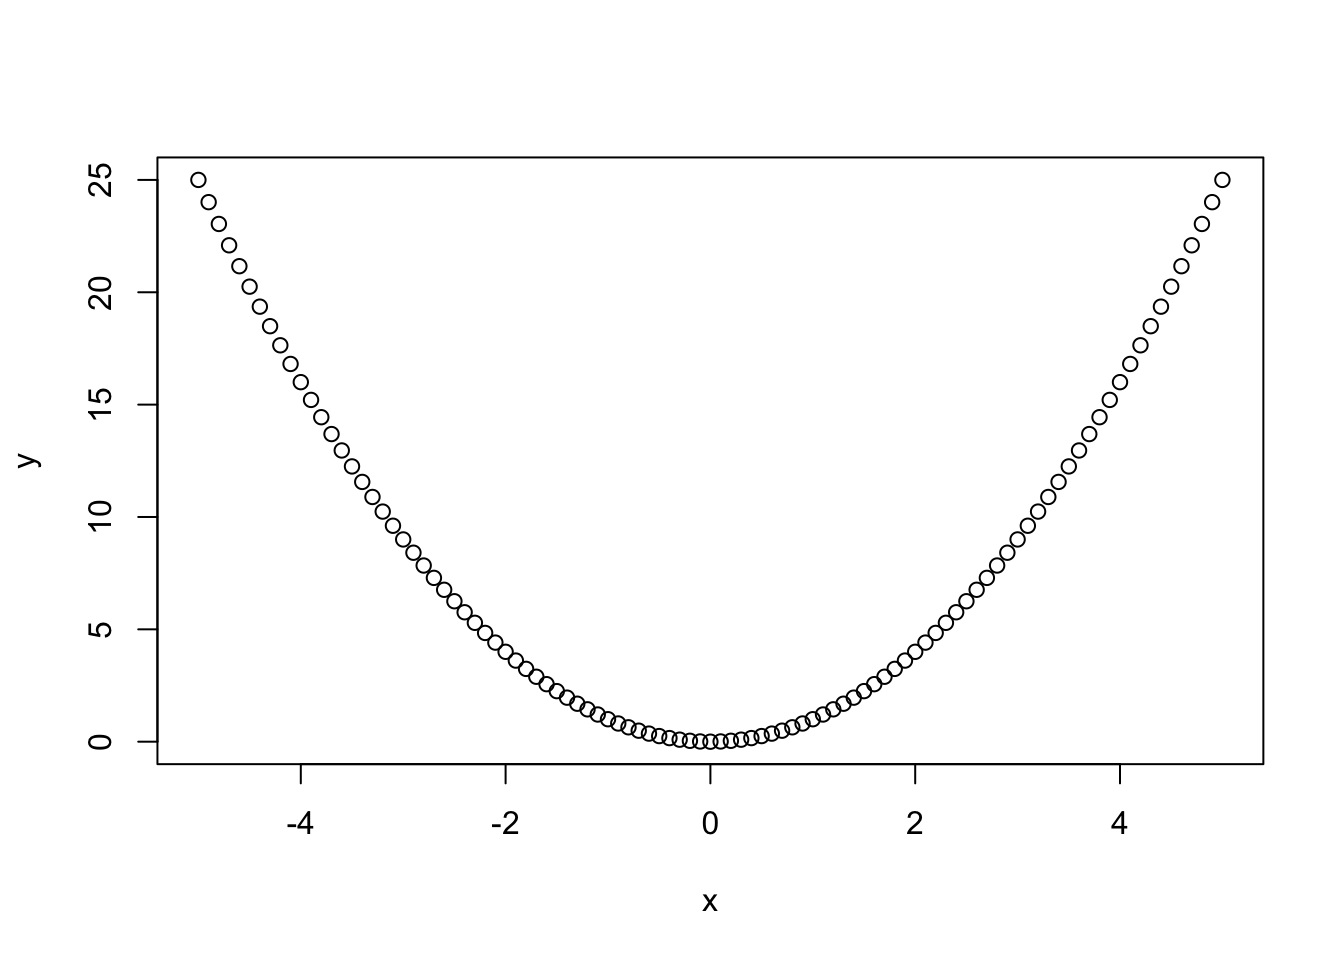
\includegraphics[width=0.5\linewidth]{RMarkdown_files/figure-latex/chart_output4-1} \end{center}

Of course, all chunk options can also be modified globally.

\hypertarget{images-and-r-markdown}{%
\section{Images and R Markdown}\label{images-and-r-markdown}}

\hypertarget{images-with-knitr}{%
\subsection{Images with Knitr}\label{images-with-knitr}}

\begin{quote}
\href{https://www.lynda.com/RStudio-tutorials/Inserting-images-include_graphics/699348/2800215-4.html?srchtrk=index\%3a1\%0alinktypeid\%3a2\%0aq\%3ar+markdown\%0apage\%3a1\%0as\%3arelevance\%0asa\%3atrue\%0aproducttypeid\%3a2}{Lynda
7.1}
\end{quote}

If you know the directory to your image, you can use
\texttt{include\_graphics()} from the \texttt{knitr} package to output
the image as a figure. It will be responsive to chunk figure options.

\begin{Shaded}
\begin{Highlighting}[]
\NormalTok{knitr}\OperatorTok{::}\KeywordTok{include_graphics}\NormalTok{(}\StringTok{"images/Rlogo.svg"}\NormalTok{)}
\end{Highlighting}
\end{Shaded}

\begin{center}
\includegraphics[width=0.2\linewidth]{images/Rlogo} \end{center}

\hypertarget{images-with-raw-html}{%
\subsection{Images with Raw HTML}\label{images-with-raw-html}}

\begin{quote}
\href{https://www.lynda.com/RStudio-tutorials/Inserting-images-using-raw-HTML/699348/2800216-4.html?srchtrk=index\%3a1\%0alinktypeid\%3a2\%0aq\%3ar+markdown\%0apage\%3a1\%0as\%3arelevance\%0asa\%3atrue\%0aproducttypeid\%3a2}{Lynda
7.2}
\end{quote}

With even no understanding of HTML, inserting images is very simple.
HTML can be pasted directly into an R Markdown file.

\begin{verbatim}
<img src = "images/Rlogo.svg" width = "20%">
\end{verbatim}

The image can easily be centred with the centre tag.

\begin{verbatim}
<center> <img src = "images/Rlogo.svg" width = "20%"> </center>
\end{verbatim}

HTML images are extremely tweakable, but require knowledge of HTML!

\hypertarget{images-with-raw-latex}{%
\subsection{Images with Raw LaTeX}\label{images-with-raw-latex}}

\begin{quote}
\href{https://www.lynda.com/RStudio-tutorials/Inserting-images-using-raw-LaTeX/699348/2800217-4.html?srchtrk=index\%3a1\%0alinktypeid\%3a2\%0aq\%3ar+markdown\%0apage\%3a1\%0as\%3arelevance\%0asa\%3atrue\%0aproducttypeid\%3a2}{Lynda
7.3}
\end{quote}

\hypertarget{images-found-by-url}{%
\subsection{Images found by URL}\label{images-found-by-url}}


\end{document}
